Spoofax is a platform that allows for giving a completely
\emph{declarative} definition of a programming language and accompanying
IDE support~\cite{Kats10a}. Such a platform is called a \emph{language
workbench}. The definition of a programming language is done using
high-level \emph{meta-languages} for each aspect of the programming
language.

To define a language declaratively means that one uses the
meta-languages to specify \emph{what} the properties of a language are, not
\emph{how} these properties are implemented. For example, instead of asking
\emph{​``How do I implement a tokenizer and parser for my language?''​}, one
asks \emph{​``What is the syntax of my language?''​}. From such a description
in a meta-language, the tokenizer and parser can be derived without
the designer of the language ever having to care about its
implementation.

This section goes over the aspects that come into play with the
development of a language and how Spoofax tackles each of these
aspects. First, the section goes over the elements that make up the
specification of a language\footnote{This section follows
the structure of the language specification portion of the compiler
construction course at the TU Delft. The slides can be found here:
\url{http://tudelft-in4303.github.io/lectures/specification/}.}. A language
specification consists of the following conceptual steps:

\begin{enumerate}
\item \hyperref[ssec:syntax-def]{Syntax Definition}: The first step defines what textual
representations of a program are syntactically valid. A parser
provides an implementation of this definition, by mapping a textual
representation of a program to an abstract syntax tree (AST)
representation. In Spoofax, the syntax is declared with a domain
specific language (DSL) called SDF.
\item \hyperref[ssec:static-analysis]{Static Semantics}: The AST then goes through static analysis (type
checking, name binding and variable scoping), to test if the
program is well-formed. Static semantics describe the rules for the
static analysis step. Spoofax provides two DSLs that can specify the two
distinct parts of this step: the TS Type Specification language and
the NaBL name binding language.
\item \hyperref[ssec:term-rewrite]{Term Rewriting and Program Transformation}: Optionally, a
well-formed AST can then be transformed, for example for desugaring
or optimization. Spoofax provides Stratego for this step.
\item \hyperref[ssec:dynamic-semantics]{Dynamic Semantics}: Next the optionally transformed AST is either
compiled or interpreted, thereby providing a means of
execution. Dynamic semantics define what the behaviour is of a
program upon execution. In Spoofax, the dynamic semantics can be
defined with either Stratego or a DSL called DynSem.
\end{enumerate}

This section concludes with a discussion on the other
aspect of a language: its integrated development environment
(IDE). Spoofax provides IDE support by means of its Editor Services.

\subsection{Syntax Definition}
\label{ssec:syntax-def}
The first part of the specification of a language is its syntax. The
syntax of a language is often specified by means of a \emph{lexical
grammar} and a \emph{context-free grammar}, as can be seen in the
specification of, for example, Standard ML~\cite{Milner97}. The
lexical grammar is most often defined using regular expressions. It
defines the individual words made up of characters, such as
identifiers and numeric constants. The context-free grammar then
defines syntactically valid sentences made up of words.

\subsubsection{SDF3: syntax definition in Spoofax}
\label{ssec:orgheadline1}
To specify a syntax definition declaratively in Spoofax, a DSL called
\emph{SDF3}~\cite{Vollebregt12} is used.  SDF3 is the third generation
of the \emph{Syntax Definition Formalism} (SDF)~\cite{Heering89}. It
uses only context-free grammer productions for the specification of
both the lexical syntax and the context-free syntax, a feature that
was introduced in SDF2~\cite{Visser97}.

The declarative nature of SDF3 allows for thinking in terms of the
structure (the \emph{what}), instead of in terms of parser algorithms (the
\emph{how}) as is the case with many current parser generators such as
ANTLR and YACC~\cite{Kats10b}. The syntax definition is used to
make parsers that parse a textual representation of a program into its
AST and pretty-printers for mapping ASTs back to text. However, due to
its declarative nature, SDF3 is not limited to generating parsers and
pretty printers: it can also be used for error recovery
rules~\cite{deJonge12}, syntax highlighting rules and folding
rules for editors (see \cref{ssec:editor-serv}).

The Spoofax API gives access to the generated parser through the
\texttt{SyntaxService}.

\subsubsection{AST-based rules}
\label{ssec:orgheadline2}
The meta-languages that will be discussed in the coming sections all
have one property in common: all of them use \emph{rules} based on the AST
in order to specify one of the parts of a language definition. The
rules are said to be \emph{syntax-directed}: the specification for one AST
node (whether it be a static semantics, rewriting or dynamic semantics
specification) is done by the specification of the children of that
AST node~\cite{Winskel93}.

\subsection{Static Semantics}
\label{ssec:static-analysis}
Static semantics refer to the meaning of what a well-formed program is
for a particular language~\cite{Milner97}. This imposes more
constraints than syntax definition, such as name binding, scoping
rules and type checking. These cannot be specified by a syntax
definition alone and are thus considered separately.

\subsubsection{Declarative static semantics specification in Spoofax}
\label{ssec:orgheadline3}
In Spoofax, all the static semantics as well as the dynamic semantics
used to be specified with the \emph{Stratego} transformation language
(which is discussed in \cref{ssec:term-rewrite}). Nowadays, two
high-level DSLs exist for specifying static semantics declaratively:
NaBL and TS. The two DSLs can work together: for instance, the type of
a variable can be set with NaBL, so that TS can be used to make
assertions on the type of that variable.

The static analysis step of a language is exposed through the Spoofax
API by the \texttt{AnalysisService}.

\subsubsection{NaBL: the Name Binding Language}
\label{ssec:nabl}
With \emph{NaBL} (pronounced \emph{enable}), name binding and scoping can be
specified declaratively using AST-based
rules~\cite{KonatKWV12}. Here is an example of name binding
and scoping rules for a class, from the \emph{paplj}
language.\footnote{paplj is used as an exercise language for the
``Declare Your Language'' book, which is a work-in-progress at the time
of writing. More information can be found here:
\url{https://github.com/MetaBorgCube/declare-your-language}}
\lstset{language=nabl,numbers=left}
\begin{lstlisting}
namespaces Program Class Field Method Variable
// ...
binding rules
  Class(c, _, _, _) :
    defines Class c of type ClassT(c)
    // Declare new scope
    scopes Field, Method, Variable
    implicitly defines Variable This() of type ClassT(c)

  Extends(c) :
    // Import namespaces from superclass
    imports Field, Method from Class c
\end{lstlisting}
The most important concept to take away from this example is the way
the rules are specified on the AST: new scopes for names can be
defined on the level of an AST node, and can be imported again by
referring back to the scope definition.

As can be seen from line 8, it can also associate type information
with names to interplay with TS. The type annotations can also be used
for instance when desugaring or rewriting with Stratego (see \cref{ssec:term-rewrite}).

\subsubsection{TS: the Type Specification language}
\label{ssec:orgheadline4}
Type checking can be done by specifying typing rules with the \emph{TS}
DSL. Again an example of the paplj language:
\lstset{language=type-spec,numbers=left}
\begin{lstlisting}
type rules
  Class(c1, Extends(c2), _, _) :-
    where store ClassT(c1) <sub: ClassT(c2)

  x@This() : t
    where definition of x : t
// ...
type rules
  Add(e1, e2) : NumT()
    where e1 : NumT() else error "number expected" on e1
      and e2 : NumT() else error "number expected" on e2
\end{lstlisting}
This example shows how in TS, the rules are syntax-directed: The
typing rule of the \texttt{Add} node is specified by the types of its
children \(e_1\) and \(e_2\), on which the typing rules will be applied
recursively.

Again, in line 6, interplay can be seen between TS an NaBL. Here the
type of a variable can be accessed, which is set in the NaBL
specification (see the previous subsection, \cref{ssec:nabl}).

\subsection{Term Rewriting and Program Transformation}
\label{ssec:term-rewrite}
Sometimes the AST needs some form of transformation before it is to be
compiled or executed, for example to transform it to a canonical form,
or to perform optimizations such as constant folding. Program
transformations are specified by \emph{term rewrite rules}: The left-hand
side of a rule introduces a pattern (for example \(x + x\)), and the
right-hand side specifies a replacement for it (e.g. \(2\cdot x\)).

\subsubsection{Rewriting using Stratego}
\label{ssec:orgheadline5}
Spoofax offers a DSL called \emph{Stratego} for specifying program
transformation with rewrite rules~\cite{Visser01}. Stratego can be
seen as the most general part of Spoofax: before NaBL and TS, Stratego
was used for specifying the static semantics. Moreover, being a
program transformation language, it can also serve as a compiler and
can thus be used to specify the dynamic semantics.

An example of a rewrite rule for the paplj language is given below.
\lstset{language=stratego,numbers=left}
\begin{lstlisting}
rules
  desugar-let :
  	Let([], e) -> e

  desugar-let :
  	Let([b1, b2 | bs], e) -> Let([b1], Let([b2 | bs], e))
\end{lstlisting}
This desugars a \texttt{let} expression with multiple bindings into multiple
nested \texttt{let} expressions each having just one binding. Again it can be
seen that these are syntax-directed rules, from the way the rules are
specified using the AST.

To construct the main algorithm of the program transformation,
Stratego has the notion of \emph{strategies}. A strategy is used to specify
where and in what order the rewrite rules are applied to an
AST. Another example from paplj is given below:
\lstset{language=stratego,numbers=left}
\begin{lstlisting}
strategies
  pre-desugar =
    innermost(desugar-let <+ desugar-do)

  post-desugar =
    innermost(desugar-do <+ desugar-get <+ desugar-set);
    resugar
\end{lstlisting}
The strategy \texttt{innermost} in this example is used to apply the strategy
given as parameter (a composition of rewrite rules) in a specific
traversal order on the AST nodes.

The Spoofax API provides the \texttt{TranformService} for performing program
transformation. Internally the \texttt{TransformService} accesses the
Stratego runtime, which is retrieved from the
\texttt{StrategoRuntimeService}. The same holds for the \texttt{AnalysisService} of
the previous section: it too uses the Stratego runtime.

Stratego furthermore has support for \emph{native} strategies, which are
specified in Java instead. Therefore the interface is bidirectional:
Stratego can hook into Java, and Java can use the Stratego API.

\subsection{Dynamic Semantics}
\label{ssec:dynamic-semantics}
Dynamic semantics refers to how a program written in some language
behaves~\cite{Winskel93}. There are many approaches to formally
specify the dynamic semantics of a programming language (for an
extensive treatment, see~\cite{Winskel93}). For this section only
one sort of approach called \emph{operational semantics} is relevant.

\subsubsection{DynSem: rule-based dynamic semantics}
\label{ssec:dynsem}
Aside from Stratego, the Spoofax team has developed an additional
method to declare the dynamic semantics of a language, namely a DSL
called \emph{DynSem}~\cite{VerguNV15}. DynSem allows for an operational
semantics specification from which a Java-based AST interpreter is
automatically generated.

In DynSem, like other meta-languages in Spoofax, the dynamic semantics
are specified by means of syntax-directed rules. To show how rules can
define the dynamic semantics of a language, consider the classic
example of the \(\beta\)-reduction, which defines function application in
the lambda calculus. The rule replaces all the occurences of the
parameter \(x\) with the argument \(e_2\), within the expression \(e_1\):

\begin{equation}
(\lambda x.e_1) e_2 \rightarrow e_1[x := e_2]
\end{equation}

In a similar way, dynamic semantics can be specified in DynSem using a
syntax very similar to the formal syntax used in the literature. Take
here the example of defining the behaviour of some boolean operators
in paplj:
\lstset{language=dynsem,numbers=left}
\begin{lstlisting}
rules
  And(BoolV(false), _) --> BoolV(false).
  And(BoolV(true), e)  --> e.

  Or(BoolV(true), _)  --> BoolV(true).
  Or(BoolV(false), e) --> e.
\end{lstlisting}
The example applies the standard rules for boolean operators, and is
sufficient to specify the behaviour of these operators. The rules are
recursively applied to the expression \(e\) on the right-hand side of
the rule until it eventually converges.

DynSem generated interpreters can be accessed through the same APIs as
those of Stratego, because the interpreter is a native Stratego
strategy. Therefore, alternatively, the generated interpreter can also
be accessed directly from Java provided that one has the AST of the
program to interpret.

\lstset{numbers=none}

\subsection{Editor Services}
\label{ssec:editor-serv}
This section concludes with a brief description of editor services,
which provide the IDE support for languages defined in
Spoofax. Examples of such services include an outline view, menus in
which one can bind actions to menu buttons (see
\cref{fig:menu-actions}), but also syntax highlighting, syntactic code
completion and code folding rules\footnote{More services are
listed on the Spoofax website:
\url{http://www.metaborg.org/spoofax/editor-services/}}.

The Spoofax API provides the editor services with similar naming. For
example, the outline can be retrieved from the \texttt{OutlineService}, the
syntax highlighting can be accessed through the \texttt{StylerService} and
syntactic code completion is accessed with the
\texttt{CompletionService}. The defined menus for a particular language can
be retrieved with the \texttt{MenuService}, from which the menu actions can
be retrieved and used.

\begin{figure}[htb]
\centering
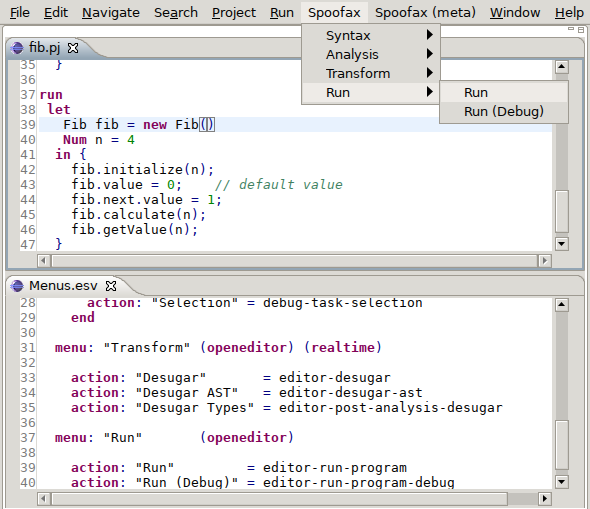
\includegraphics[width=0.6\textwidth]{./img/menu-actions.png}
\caption{\label{fig:menu-actions}
A menu action for the paplj language defined using Spoofax. The bottom window shows the menu definition, the top window shows a program written in paplj.}
\end{figure}

Editor services are defined using a DSL, shown in the bottom window of
\cref{fig:menu-actions}. In the case of menus, their actions are
specified using Stratego. Since Stratego supports native strategies,
these actions can also be specified in Java. As such, Spoofax allows
for defining arbitrarily complex IDE actions.

Many of these editor services such as syntax highlighting and code
folding rules can be derived from the syntax
definition~\cite{Kats10c} and can be further customized if
needed. Taken together with the language definition, the editor
services provide a language with a complete and state-of-the-art IDE
experience~\cite{Kats10a}.
